\section{Implementation}

Zur Bearbeitung der Problemstellung, wurde die Programmiersprache C und
überwiegend ein objektorientiertes Paradigma verwendet.  Die Implementation
besteht aus drei nahezu unabhängige Bereichen, dem Go, den neuronalen Netzen
und dem Genetischen Algorithmus. Die benötigte Funktionalität wurde jeweils als
Modul einer Bibliothek implementiert.  Diese wurde mit dem Test Framework Check
\cite{check} während der Entwicklung regelmäßig auf Fehler untersucht.

Als Schnittstelle für den Benutzer wurden kleine Anwendungen geschrieben, die
Algorithmen und Datenstrukturen aus der Bibliothek verwenden, um einzelne
Aufgaben zu erfüllen.


\subsection{Das neuronale Netz}
%Der Aufbau des Netzes, Funktionsweise von Backpropagation

Ein neuronales Netz besteht aus Neuronen, ähnlich einem menschlichen Gehirn. Die
Neuronen sind in Schichten angeordnet, den Layern des Netzes. Das erste Layer
ist dabei das Input Layer, das letzte das Output Layer. Zwischen den Layern
gehen Kanten von jedem Neuron des einen zu jedem Neuron des anderen Layers.
Diese Kanten haben Gewichte und pro Layer gibt es auch einen Bias, der zum
Kantengewicht addiert wird. Ein Signal wird durch das Input Layer aufgenommen,
durch die Layer weitergegeben und vom Output Layer wieder ausgegeben. Das
Weiterleiten innerhalb des Netzes funktioniert über die Kanten. Der Output eines
Neurons ist die Summe aller seiner Eingänge. Durch eine Sigmoidfunktion - hier
$\frac{1}{1 + e^{-x}}$ - werden diese Summen auf den Wertebereich $[-1;1]$
reduziert, wobei die Funktion gleichzeitig die spätere Anwendung des
Backpropagation Algorithmus ermöglicht. Der fertige Output des
Neurons wird dann mit den jeweiligen Kantengewichten multipliziert und an die
Neuronen des nächsten Layers weitergeleitet. Vor allem hier ist also sehr viel
zu Berechnen. 

Der Aufbau der Netze ist variabel, die Anzahl der Layer sowie die Anzahl der
Neuronen pro Layer ist frei wählbar. Das Input Layer sollte allerdings für jeden
Schnittpunkt des Eingabebrettes ein Neuron haben und das Output Layer
entsprechend ein Neuron pro Schnittpunkt plus ein Neuron um Passen anzuzeigen.
Die Ausgabe sind die Präferenzen der Netze, der Schnittpunkt mit dem höchsten
Wert wird besetzt. 

Damit die Netze zumindest die Regeln von vornherein erlernen, gibt es eine
Methode für Supervised Learning; den Backpropagation
Algorithmus. Für ihn muss bekannt sein, was das erwartete Ergebnis ist, weswegen
die Netze so nur auf die Go Regeln und nicht auf die Taktik trainiert werden
können. Der Algorithmus basiert darauf, dass der tatsächliche Ausgabewert mit
dem erwarteten Wert verglichen wird und der so ermittelte Fehler zur Korrektur
der Kantengewichte benutzt wird. Um die richtigen Korrekturwerte für die
einzelnen Layer zu erhalten, muss die Ableitung der Fehlerfunktion durch die
Ableitung des Kantengewichts berechnet werden. Dazu summiert man die
Fehlersignale der vorhergehenden Schicht mal dem dazugehörigen Kantengewicht auf
und multipliziert es mit der Ausgabe des Neurons. So wird nur der Teil des
Fehlers, der tatsächlich von diesem Neuron verursacht wurde, korrigiert. 

\subsubsection{Dateiformat}
Um die neuronalen Netze einfach wiederverwenden und übertragen zu können,
wurden einfache Dateiformate entwickelt. In diesen lassen Mengen von Netzen
entweder in menschenlesbarer Textform (Beispiel in Listing
\ref{lst:fileformat}, Seite \pageref{lst:fileformat}) oder in Binärform
abspeichern.

\subsection{Das Go-Modul}
%Welche Komponenten? Wie spielt es zusammen?

Die Regeln von Go sind hauptsächlich in dem Board Modul implementiert. Dieses
stellt einen entsprechenden Datentypen (\texttt{board\_t}) zur Verfügung,
welcher das Spielfeld repräsentiert und die momentane Stellung in seinem
Zustand speichert.  Auf das Board können Steine platziert werden. Dabei wird
überprüft, dass die Züge auch legal sind.  Das Board legt die Gruppen in einer
internen Datenstruktur ab und verbindet einen platzierten Stein mit den
benachbarten Gruppen der selben Farbe. Mit den Gruppen ist jeweils die Anzahl
der verbleibenden Freiheiten gespeichert.  Nach dem Platzieren eines Steins
wird überprüft, ob die benachbarten Gruppen des anderen Spielers ihre letzte
Freiheit durch den Zug verloren haben und geschlagen werden müssen.  Das
Speichern der Gruppen ist wichtig, da die Freiheiten sonst bei jedem Zug neu
berechnet werden müssten.
Die Berechnung des Gebiets erfolgt mit einem Flood-Fill Algorithmus.

Das Klassendiagramm (Abbildung \ref{fig:class_diagram}) gibt einen Überblick
über den Zusammenhang der erstellten Datenstrukturen. Um die neuronalen Netze
Go spielen zu lassen und dabei mit dem genetischen Algorithmus zu trainieren,
sind weitere Datenstrukturen notwendig.

Der Spielablauf einer Partie Go wird durch das Game (\texttt{game\_t})
modelliert. Dieses lässt zwei Player (\texttt{player\_t}) auf einem Board
gegeneinander spielen. Das Interface eines Player definiert eine Funktion, die,
gegeben der Zustand eines Boards, den zu spielenden Zug zurückgibt. Es werden
zwei Implementationen zur Verfügung gestellt, um entweder den Zug durch ein
neuronales Netz berechnen oder durch einen menschlichen Spieler auf der
Kommandozeile eingeben zu lassen. Während des Spielablaufes fragt das Game
abwechselnd die Player nach ihren Zügen und setzt die Steine entsprechend auf
das Board. Nach zweimaligem Passen oder bei erreichen des Zuglimits, wird das
Spiel beendet und die Punkte gezählt.
Zur weiteren Analyse eines Spiels, können Recorder (\texttt{recorder\_t}) beim
Game registriert werden. Diese können den Spielverlauf wahlweise in ASCII-Art
oder dem Smart Game Format (SGF)\cite{sgf} aufzeichnen. Letzteres wird
üblicherweise von Go-Software unterstützt, so dass sich Spiele Zug für Zug
nachverfolgen lassen.

\begin{figure}
    \centering
    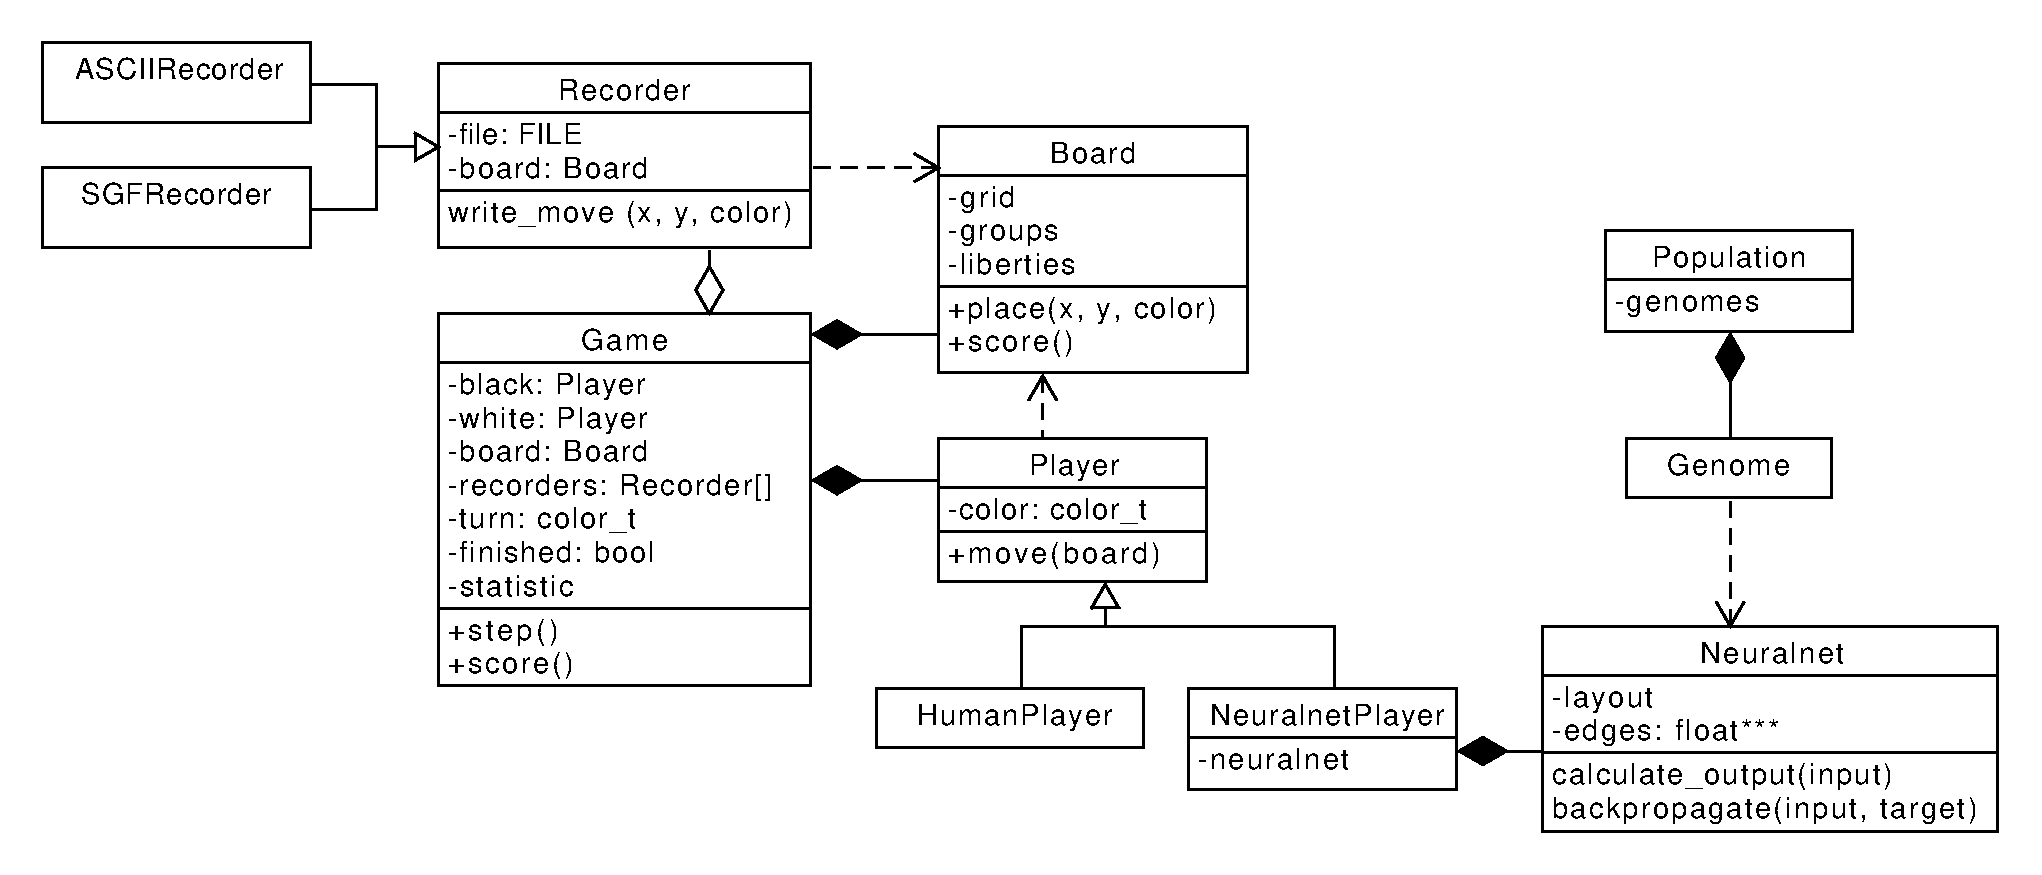
\includegraphics[width=\textwidth]{content/img/class_diagram}
    \caption{Klassendiagramm von Neugengo}
    \label{fig:class_diagram}
\end{figure}

% Die Implementation des Go Spiels besteht aus mehreren Komponenten. Zunächst
% sind die Spielregeln und grundlegenden Aktionen im Spiel, wie etwa zu passen
% oder einen Stein zu legen, in board.h, also dem Go Brett, implementiert. Das
% Brett ist darin ein eigener Datentyp, der unter anderem den aktuellen Stand
% des Spieles, etwa welcher Spieler an der Reihe ist oder ob ein Ko vorliegt,
% und alle existierenden Gruppen von Steinen inklusive deren Freiheiten
% speichert. Die Gruppen sind deshalb wichtig, weil sie beim Schlagen eines
% Steins berücksichtigt werden müssen; wären sie nicht gespeichert, müssten sie
% in jedem Zug in dem Gebiet um den neuen Stein berechnet werden, was relativ
% zeitaufwändig wäre. Es ist also, vor allem da wir unseren Fokus auf kleinere
% Netze gelegt haben, sinnvoll die Steingruppen zu speichern. 
%
% Während im Brett die meisten Regeln implementiert sind, kann es nicht
% selbstständig den Spielablauf regeln. Dafür wird game.h benutzt, worin ein Spiel
% für eine bestimmte Brettgröße und zwei Spieler erstellt wird und Schritt für
% Schritt gespielt werden kann. Die Spieler sind in player.h definiert und können
% sowohl Menschen als auch neuronale Netze sein. So muss im eigentlichen Spiel
% nicht mehr auf die Funktionen des neuronalen Netz zurückgegriffen werden, da die
% Züge über den erstellten Spieler abgefragt werden. Im Spiel kann außerdem ein
% Zuglimit gesetzt werden, für den Fall dass etwa eine Endlosschleife auftritt
% oder die Spiele besonders kurz gehalten werden sollen. 
% 
% Um die Spiele nachträglich zu analysieren, gibt es die Möglichkeit sie
% aufzuzeichnen. Dabei können zwei Formate benutzt werden: zum einen ASCII-Art,
% zum anderen SGF. ASCII-Art kann natürlich ohne zusätzliche Software sofort
% genutzt werden, um die SGF Dateien sinnvoll zu nutzen wird aber ein geeignetes
% Programm benötigt. Viele Go Programme etwa sind in der Lage SGF Dateien
% einzulesen und dann Zug für Zug darzustellen. 

\subsection{Der genetische Algorithmus}
%Wie funktioniert er?

Der genetische Algorithmus (Algorithmus \ref{alg:genetic}) imitiert die
Evolution um die Spielstärke der neuronalen Netze zu verbessern. Entsprechend
wird auch Terminologie aus der Biologie übernommen: Population, Genom
Mutation, Generation, Fitness. Eine Generation bezeichnet dabei eine Abfolge
von Spielen und die Selektion und Mutation der Population. Die Anzahl dieser
Generationen wird anfangs festgelegt.

Jedes Netz stellt hierbei ein Individuum einer Population dar, wobei
dessen Fitnesswert davon abhängt, wie viele Spiele dieses Individuum
in einer Generation gewonnen hat. Soll die Population eine
Generation voran gebracht werden, wird zunächst ausgewählt, welche Individuen in
die nächste Generation übernommen werden. Sie werden zufällig ausgesucht,
allerdings ist die Wahrscheinlichkeit ein Netz zu wählen proportional zu seinem
Fitnesswert. Ist ein Netz also besonders fit, wird es wahrscheinlicher in der
nächsten Generation auftauchen. Um keine guten Netze durch "Pech" bei der 
zufälligen Selektion zu verlieren, werden zusätzlich (in unserem Fall 4) Plätze 
in der nächsten Generation reserviert, die mit den unabgeänderten besten Netzen 
der letzten Generation gefüllt werden. Danach werden die Netze mutiert, 
ebenfalls zufällig. Es gibt eine bestimmte Mutationswahrscheinlichkeit, mit 
deren Hilfe überprüft wird, ob ein bestimmtes Kantengewicht mutiert, also um einen
zufälligen Wert verändert werden soll, oder nicht. Für jedes Element des Genoms
wird eine Zufallszahl zwischen 0 und 1 erzeugt, ist sie kleiner als die
Mutationswahrscheinlichkeit, dann wird mutiert. Ist dieser Schritt abgeschlossen, 
ist die Population eine Generation fortgeschritten. Nun muss die Fitness jedes Netzes
durch Spiele gegen andere aktualisiert werden, sodass der Algorithmus 
wieder von vorne anfangen kann.

\begin{algorithm}
    \caption{Genetischer Algorithmus}
    \label{alg:genetic}
    \begin{algorithmic}[1]
        \Require Eingabedatei $in\_file$, Iterationen $n$
        \Ensure Ausgabedatei $out\_file$
        \State $N_0 \gets$ \Call{load\_nets}{$in\_file$}
        \For {generation $i = 0$ to $n$}
            \State $wins \gets (0, 0, \ldots, 0)$
            \For {$\forall net_a \neq net_b \in N_i$}
                \State \Call{play\_game}{$net_a, net_b$}
                \If {$net_a$ won the game}
                    \State $wins[net_a] \gets wins[net_a] + 1$
                \Else
                    \State $wins[net_b] \gets wins[net_b] + 1$
                \EndIf
            \EndFor
            \State $N_{i+1} \gets$ \Call{the\_next\_generation}{$N_i, wins$}
        \EndFor
        \State \Call{save\_nets}{$out\_file$}
    \end{algorithmic}
\end{algorithm}

\subsection{Die Benutzerschnittstelle}
\begin{samepage}
Die Benutzerschnittstelle von Neugengo besteht aus mehreren Command Line Tools,
die folgende Funktionen abdecken:
\begin{itemize}
    \item Erstellung von neuronalen Netzen
    \item Training von neuronalen Netzen mittels Backpropagation
    \item Training von neuronalen Netzen mittels genetischen Algorithmus
    \item Auswertung von Netzen gegeneinander
    \item Ausführung von Mensch-gegen-Netz-Spielen
\end{itemize}
\end{samepage}

Das \texttt{ngg\_tool} implementiert Funktionen zum zufälligen Erstellen von
neuronalen Netzen eines gegebenen Layouts. Weiterhin lassen sich Trainingsdaten
generieren, die einer Situation eines Go-Brettes entsprechen. Diese lassen sich
verwenden, um die neuronalen Netze mit Backpropagation zu trainieren.
Listing \ref{lst:ngg_tool-help} (Seite \pageref{lst:ngg_tool-help}) zeigt das
Command Line Interface.

\texttt{ngg\_game} unterzieht eine Menge von neuronalen Netzen einem
unsupervised Training mit dem genetischen Algorithmus. Nach einer angegebenen
Anzahl an Iterationen oder des Empfangens des Signals \texttt{SIGUSR1} werden
die neuen bzw. geänderten Netze gespeichert.
Siehe Listing \ref{lst:ngg_game-help} (Seite \pageref{lst:ngg_game-help}).

\texttt{ngg\_test} kann benutzt werden, um zwei Sets an Netzen gegeneinander
spielen zu lassen, wobei jedes Netz zweimal gegen jedes aus dem gegnerischen
Set (einmal als Weiß, einmal als Schwarz) spielt. Die Ausgabe enthält die Summe
aller Punkte, die beide Sets erzielt haben. Auf diese Weise lassen sich einzelne
Netze oder ganze Populationen auf deren Stärke prüfen. 

Mit \texttt{ngg\_hvsai} lassen sich interaktive Spiele gegen abgespeicherte
neuronale Netze spielen. Das Spielfeld wird durch ASCII-Art repräsentiert
(Abbildung \ref{fig:ngg_hvsai}). Über eine mit Readline \cite{readline}
realisierte Eingabe wird eine Position abgefragt, auf diese, falls erlaubt,
gesetzt wird. Anschließend wird durch das gewählte neuronale Netz der Zug des
Gegners berechnet.

\begin{figure}
    \centering

    \begin{subfigure}[t]{0.45\textwidth}
        \begin{lstlisting}[%
            numbers=none,
        ]
  0 1 2 3 4 5 6 7 8 
0 + + + + + + + + + 0
1 + + + + + + + + + 1
2 + + + + + + + + + 2
3 + + + B + + + + + 3
4 + + + + + + + + + 4
5 + + + + + + + + + 5
6 + W + + + + + + B 6
7 + + + + + B + B W 7
8 + + + + + W + W + 8
  0 1 2 3 4 5 6 7 8 

You are black.

Enter x-position (0-8,p): 8
Enter y-position (0-8,p): 8
        \end{lstlisting}
        \caption{vor einem Zug}
    \end{subfigure}
    \quad
    \begin{subfigure}[t]{0.35\textwidth}
        \begin{lstlisting}[%
            numbers=none,
            showlines,
        ]
  0 1 2 3 4 5 6 7 8 
0 + + + + + + + + + 0
1 + + + + + + + + + 1
2 + + + + + + + + + 2
3 + + + B + + + + + 3
4 + + + + + + + + + 4
5 + + + + + + + + + 5
6 + W + + + + + + B 6
7 + + + + + B + B + 7
8 + + + + + W + W B 8
  0 1 2 3 4 5 6 7 8 




 
        \end{lstlisting}
        \caption{nach einem Zug}
    \end{subfigure}
    \caption{Ausschnitt aus einem interaktivem Spiel mit \texttt{ngg\_hvsai}}
    \label{fig:ngg_hvsai}
 \end{figure}

Im Allgemeinen sieht die vorgesehene Nutzung also wie folgt aus: Zuerst werden
neuronale Netze und Trainingsdaten erstellt.  Dann wird Backpropagation
angewandt, um die Netze mit Hilfe der Trainingsdaten zu trainieren.
Anschließend können die resultierenden Netze beliebig oft und lange durch den
genetischen Algorithmus trainiert werden. Die Ergebnisse werden zur weiteren
Verwendung in Dateien abgespeichert.
Zur Überprüfung wie erfolgreich das Training verlaufen ist, kann man Netze
gegen andere gespeicherte oder zufällig generierte Netze antreten lassen.
Weiterhin kann interaktiv gegen die trainierten Spieleauf gespielt werden.
